% Section 5.1
\section{Analysis and Discussion}\label{sec:analisis-discusion}

Our interest in identifying and classifying studies related to HTCondor universes that impact the domains of distributed and parallel computing, HTC, software development, virtualization and microservices, computer networks, computational infrastructure, artificial intelligence, data analysis, computational thinking, among others, and that also contribute to the academic dimensions of teaching, research, and outreach, was focused toward the creation and presentation of a taxonomy.

Through the proposed taxonomy, we contribute to the documentary organization of these domains. See Figure~\ref{fig:taxonomia}. One way to use it is to facilitate the identification and classification of studies related to HTCondor universes for purposes related to those of this SMS. Additionally, domains in which the SPSs resulting from this mapping are classified can be evidenced, which could be taken as a sample, resulting from a structured process, of the state of the art around this topic, thus allowing rapid location of relevant studies in certain areas, in addition to a quick summary of some of the domains related to HTCondor.

\begin{figure}[htbp]
    \centering
    \vspace{10pt}
    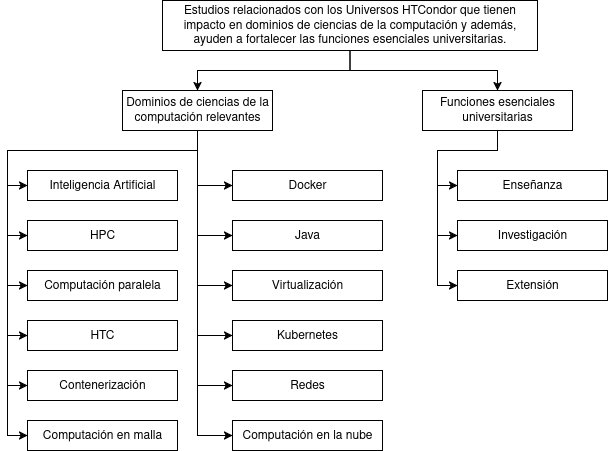
\includegraphics[scale=0.4]{resources/figures/sms-taxonomia.drawio.png}
    \vspace{6pt}
    \caption{Taxonomy of topics identified in this SMS.}
    \label{fig:taxonomia}
\end{figure}